\documentclass[a4paper]{report}
\usepackage[italian]{babel}
\usepackage[utf8]{inputenc}
\usepackage{hyperref, graphicx, colortbl, gensymb}

\hypersetup{colorlinks=false, urlcolor=black, linkcolor=black}

\title{Ingegneria del Software \\ Software  per il monitoraggio di un reparto di terapia intensiva}
\author{Matteo Meneghetti\hspace{0.2cm}VR401958 \\  Stefano Cattonar\hspace{0.2cm}VR402549}

\date{Luglio 2019}

\begin{document}

\maketitle
\tableofcontents

\chapter*{Introduzione}
    L'esame del corso di Ingegneria del Software richiedeva lo sviluppo di un software applicativo da parte di gruppi di studenti, con la possibilità di scegliere tra tre possibili progetti.\\
    Noi abbiamo deciso di sviluppare il progetto riguardante il monitoraggio di un reparto di terapia intensiva di un ospedale.
    
\chapter{Requisiti}
    \section{Casi d'uso}
        \subsection{Attori e casi d'uso}
            Come esplicitato dai requisiti gli attori del sistema sono i seguenti:
            \begin{itemize}
                \item \textbf{Gli Utenti non autenticati}\\Che possono:
                    \begin{itemize}
                        \item Visualizzare lo stato dei pazienti
                        \item Autenticarsi
                    \end{itemize} 
                \item \textbf{Il personale medico:}\\Che può:
                    \begin{itemize}
                        \item Scrivere prescrizioni
                        \item Fermare allarmi
                        \item Inserire la diagnosi di ingresso di un paziente
                    \end{itemize}
                \item \textbf{Il personale infermieristico}\\Che può:
                    \begin{itemize}
                        \item Inserire i nuovi ricoverati
                        \item Somministrare farmaci
                    \end{itemize}
                \item \textbf{Il Primario:}\\Che può:
                    \begin{itemize}
                        \item Fare tutto quello che può fare un medico
                        \item Visualizzare il report settimanale
                        \item Dimettere un paziente
                    \end{itemize}
            \end{itemize}
            
            \begin{figure}[htbp]
                \centering
                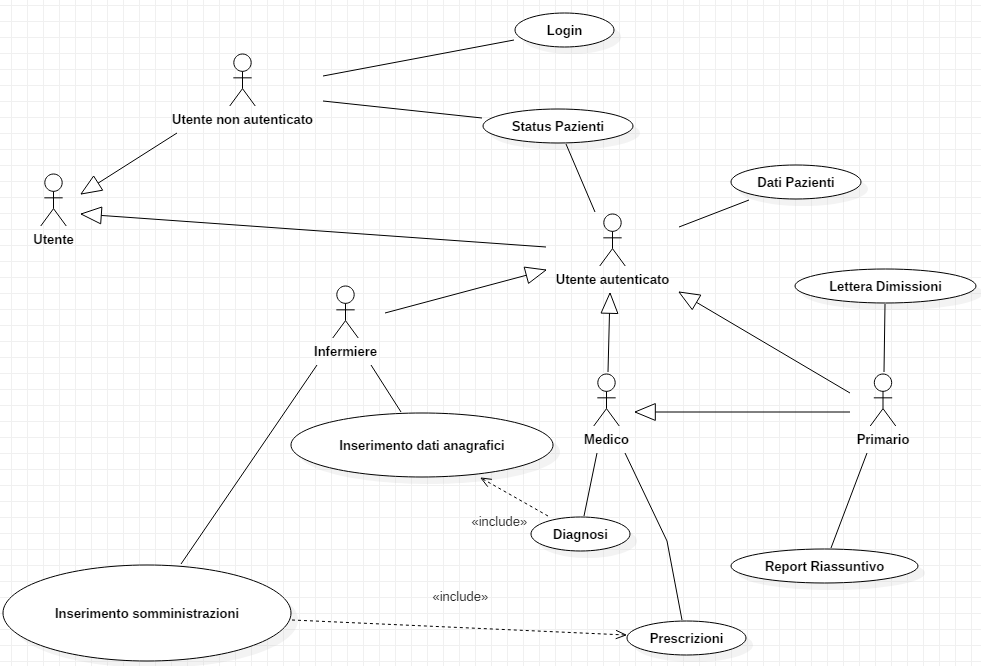
\includegraphics[scale=0.6]{USE.png}
                \caption{Diagramma dei casi d'uso}
            \end{figure}
        
        \newpage
        \subsection{Use case speciale: Visualizzare lo status dei pazienti}
            Questo caso d'uso è particolare poiché è accessibile a chiunque e non ci sono azioni da eseguire.
            \begin{table}[htbp]
                \centering
                \begin{tabular}{|c|c|}
                    \hline
                    Attori & Tutti \\\hline
                    Precondizione & Nessuna \\\hline
                    Sequenza & Nessuna \\\hline
                    Post-condizione & Nessuna \\\hline
                \end{tabular}
        \end{table}
        
        \newpage
        \subsection{Casi d'uso degli utenti non autenticati}
            \subsubsection{Login}
                Il login permette ad un utente non autenticato di autenticarsi:
                \begin{table}[htbp]
                    \begin{tabular}{|c|l|}
                        \hline
                        Attori & Utenti non autenticati \\\hline
                    Precondizione & Nessuna \\\hline
                     & 1)L'utente preme sul pulsante "Login" \\
                    Sequenza & 2)L'utente inserisce username e password \\
                      & 3)L'utente preme sul tasto "Conferma" \\\hline
                    Post-condizione & Utente autenticato \\\hline
                    \end{tabular}
                \end{table}
                \begin{figure}[htbp]
                \centering
                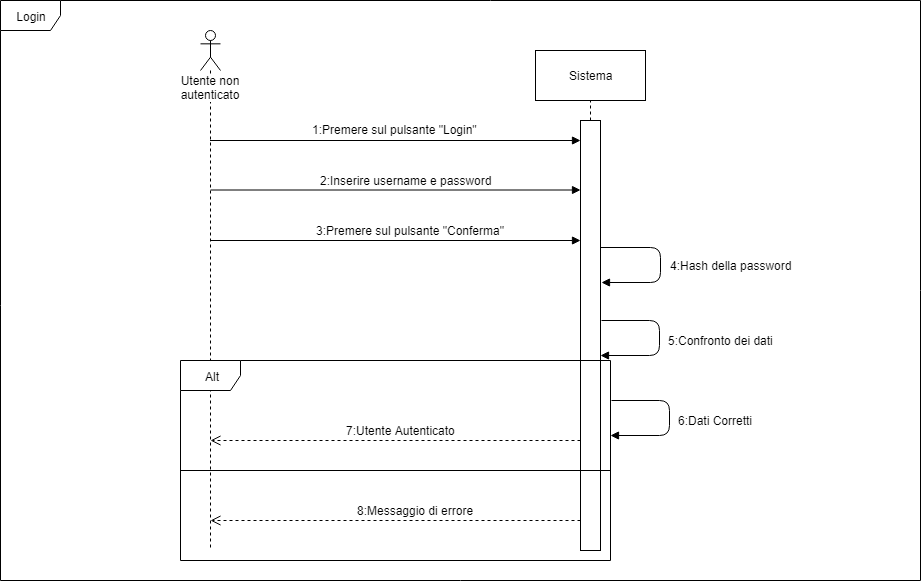
\includegraphics[scale=0.4]{LoginDia.png}
                \caption{Diagramma dei casi d'uso}
            \end{figure}
            
        \newpage
        \subsection{Casi d'uso del personale infermieristico}
            \subsubsection{Inserimento dati anagrafici}
                Il personale infermieristico deve poter compilare i dati anagrafici dei pazienti al momento del ricovero:
                \begin{table}[htbp]
                    \begin{tabular}{|c|l|}
                        \hline
                        Attori & Personale infermieristico \\\hline
                    Precondizione & L'utente deve essere autenticato \\\hline
                     & 1)L'utente preme sul pulsante "Nuovo Paziente" \\
                    Sequenza & 2)L'utente inserisce i dati anagrafici del paziente \\
                      & 3)L'utente preme sul tasto "Conferma" \\\hline
                    Post-condizione & Aggiunta del paziente e inizio monitoraggio  \\\hline
                    \end{tabular}
                \end{table}
                \begin{figure}[htbp]
                \centering
                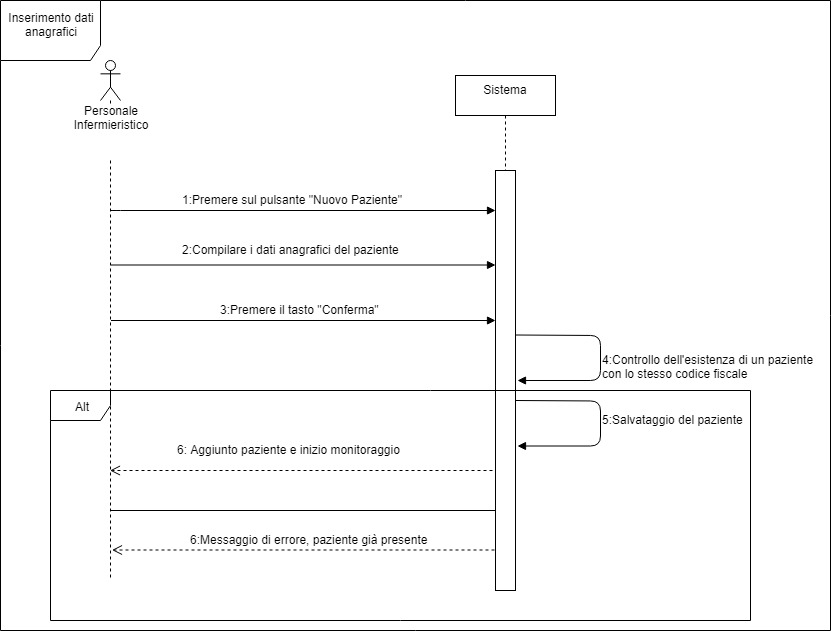
\includegraphics[scale=0.4]{InsAn.jpg}
                \caption{Sequence diagram Anagrafica}
            \end{figure}
            
        \newpage
        \subsubsection{Somministrazioni}
            Il personale infermieristico deve registrare ogni somministrazione di qualunque sostanza prescritta ai pazienti:
            \begin{table}[htbp]
                    \begin{tabular}{|c|l|}
                        \hline
                        Attori & Personale infermieristico \\\hline
                    Precondizione & L'utente deve essere autenticato \\\hline
                     & 1)L'utente preme sul pulsante "Aggiungi somministrazione" \\
                    Sequenza & 2)L'utente seleziona il paziente, il farmaco e il numero di dosi \\
                      & 3)L'utente preme sul tasto "Conferma" \\\hline
                    Post-condizione & Aggiunta della somministrazione  \\\hline
                    \end{tabular}
                \end{table}
            \begin{figure}[htbp]
                \centering
                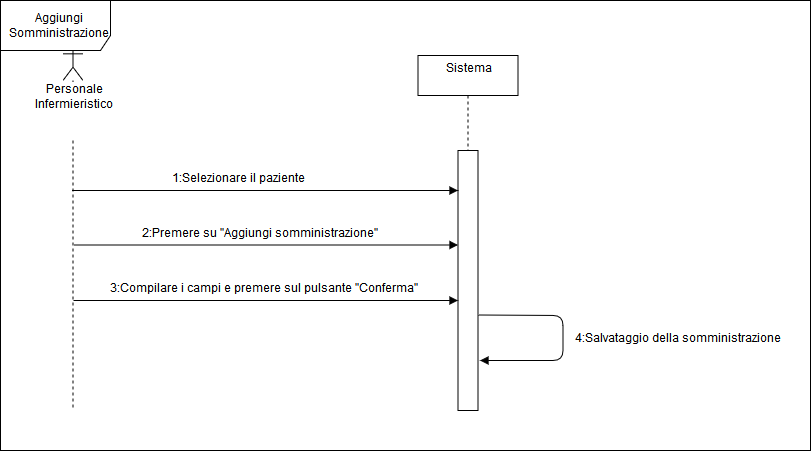
\includegraphics[scale=0.4]{InsSom.png}
                \caption{Sequence diagram Somministrazioni}
            \end{figure}
            
        \newpage
        \subsection{Casi d'uso personale medico}
            \subsubsection{Diagnosi di ingresso}
                Il personale medico quando un paziente viene registrato deve inserire all'interno della cartella clinica la diagnosi:
                \begin{table}[htbp]
                    \begin{tabular}{|c|l|}
                        \hline
                        Attori & Personale medico \\\hline
                    Precondizione & L'utente deve essere autenticato e il paziente deve essere registrato \\\hline
                     & 1)L'utente seleziona il paziente \\
                    Sequenza & 2)L'utente preme sul pulsante "Diagnosi" \\
                      & 3)L'utente compila la diagnosi e preme "Conferma" \\\hline
                    Post-condizione & Aggiunta della diagnosi  \\\hline
                    \end{tabular}
                \end{table}
                 \begin{figure}[htbp]
                    \centering
                     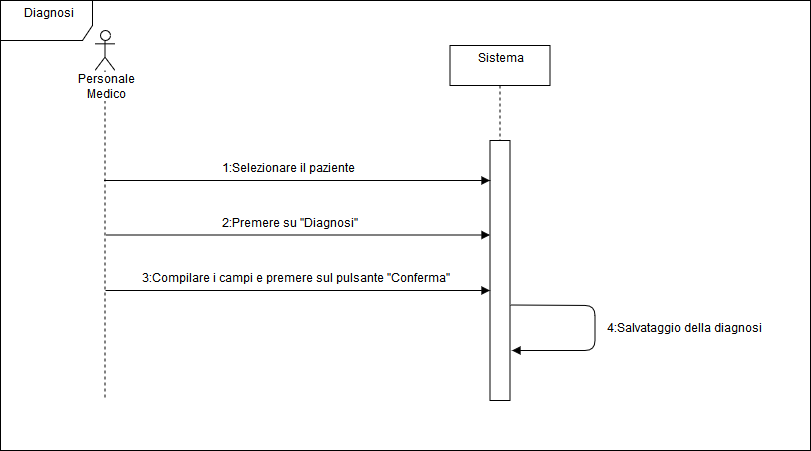
\includegraphics[scale=0.4]{Diagnosi.png}
                        \caption{Sequence diagram Diagnosi}
                \end{figure}
                
                
            \newpage
            \subsubsection{Nuova Prescrizione}
                Il personale medico deve poter inserire nuove prescrizioni di sostanze per i pazienti:
                 \begin{table}[htbp]
                    \begin{tabular}{|c|l|}
                        \hline
                        Attori & Personale medico \\\hline
                    Precondizione & L'utente deve essere autenticato e il paziente deve essere registrato \\\hline
                     & 1) L'utente seleziona il paziente \\
                    Sequenza & 2)L'utente preme sul pulsante "Aggiungi prescrizione" \\
                      & 3)L'utente compila e preme sul tasto "Conferma" \\\hline
                    Post-condizione & Aggiunta della prescrizione \\\hline
                    \end{tabular}
                \end{table}
                \begin{figure}[htbp]
                    \centering
                     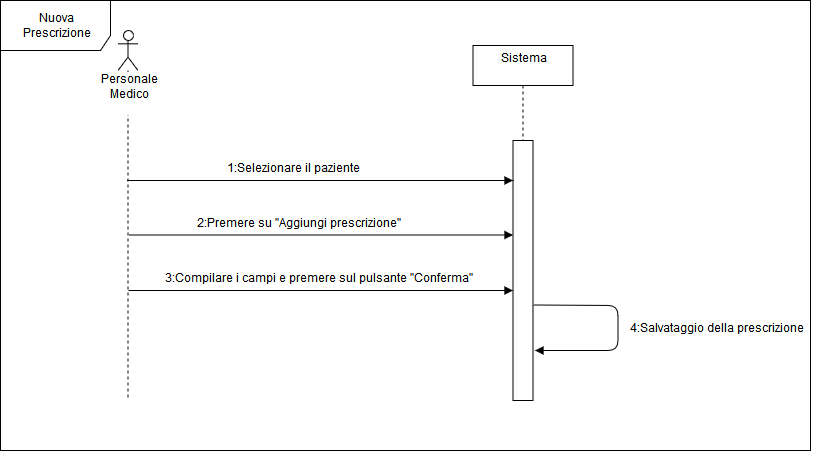
\includegraphics[scale=0.4]{InsPres.png}
                        \caption{Sequence diagram Prescrizioni}
                \end{figure}
                
        \newpage
        \subsection{Casi d'uso del primario}
            Il primario eredita tutti i casi d'uso del personale medico(di cui fa parte) in può possiede alcuni use case specifici:
            \subsubsection{Dimissioni paziente}
                Il primario può dimettere un paziente scrivendo una lettera di dimissione:
               \begin{table}[htbp]
                    \begin{tabular}{|c|l|}
                        \hline
                        Attori & Primario \\\hline
                    Precondizione & L'utente deve essere autenticato e il paziente deve essere registrato \\\hline
                     & 1)L'utente preme sul pulsante "Dimissioni" \\
                    Sequenza & 2)L'utente redige la lettera di dimissioni \\
                      & 3)L'utente preme sul tasto "Conferma" \\\hline
                    Post-condizione & Il paziente viene rimosso   \\\hline
                    \end{tabular}
                \end{table}
                \begin{figure}[htbp]
                    \centering
                     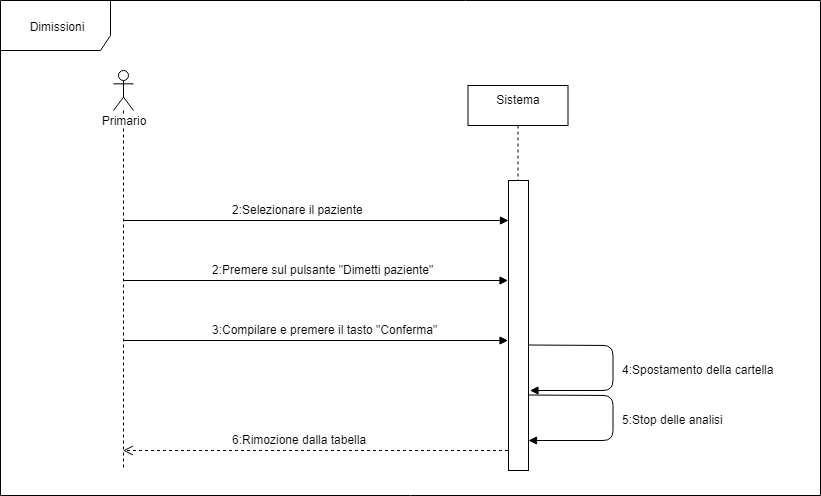
\includegraphics[scale=0.4]{Dimissioni.png}
                        \caption{Sequence diagram Dimissioni}
                \end{figure}
    \section{Activity diagrams}
        \subsection*{Login}
        \begin{center}
                    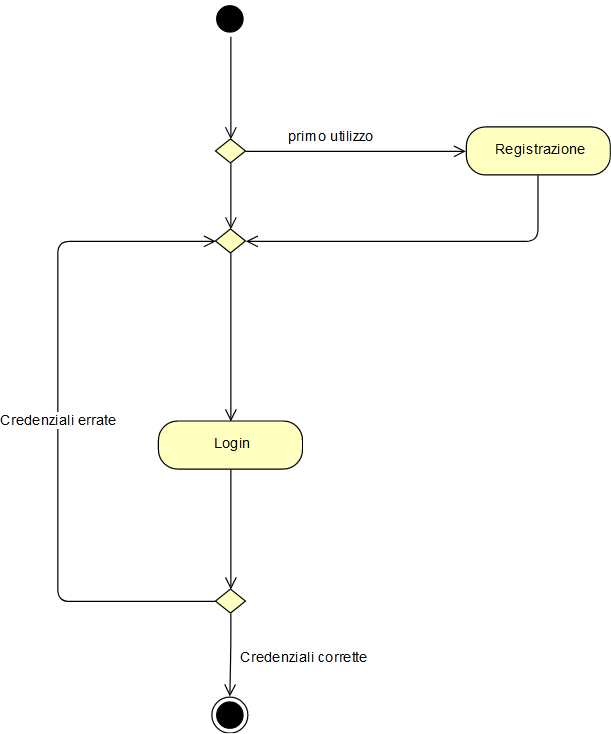
\includegraphics[scale=0.5]{activity/LoginActivity.png}
        \end{center}
        \subsection*{Infermiere}
        \begin{center}
                    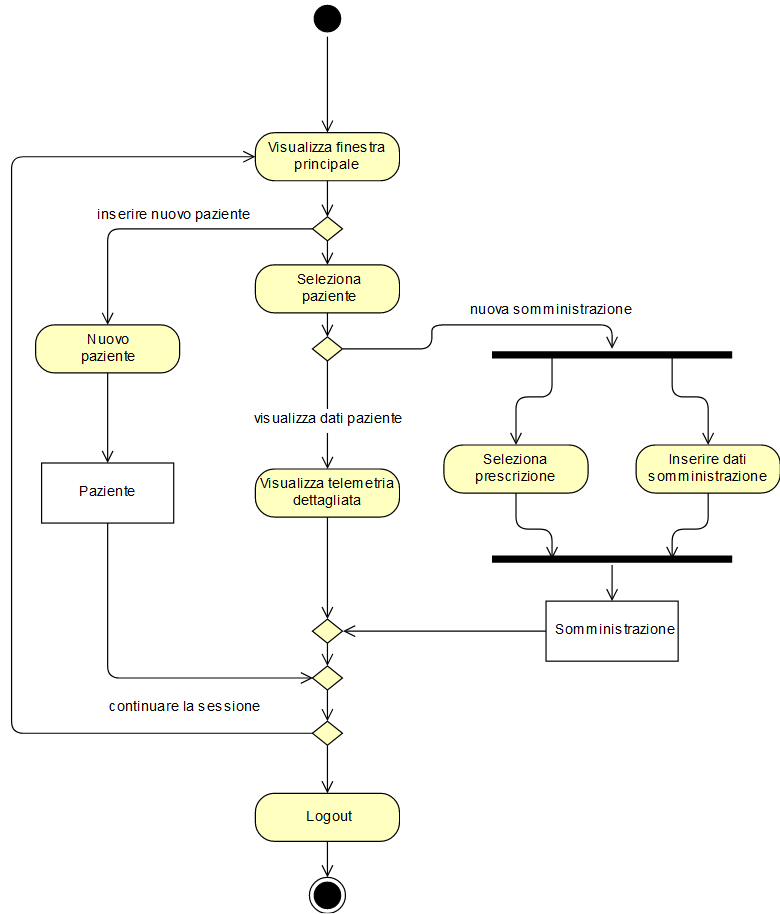
\includegraphics[scale=0.5]{activity/InfermiereActivity.png}
        \end{center}
        \subsection*{Medico}
        \begin{center}
                    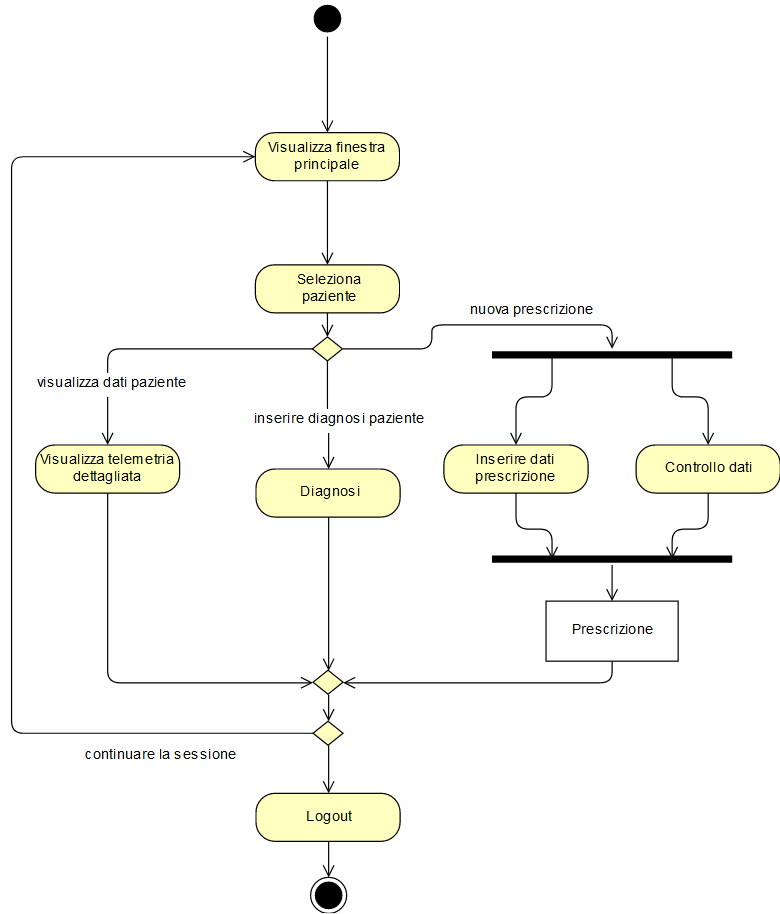
\includegraphics[scale=0.5]{activity/MedicoActivity.png}
        \end{center}
        \subsection*{Primario}
        \begin{center}
                    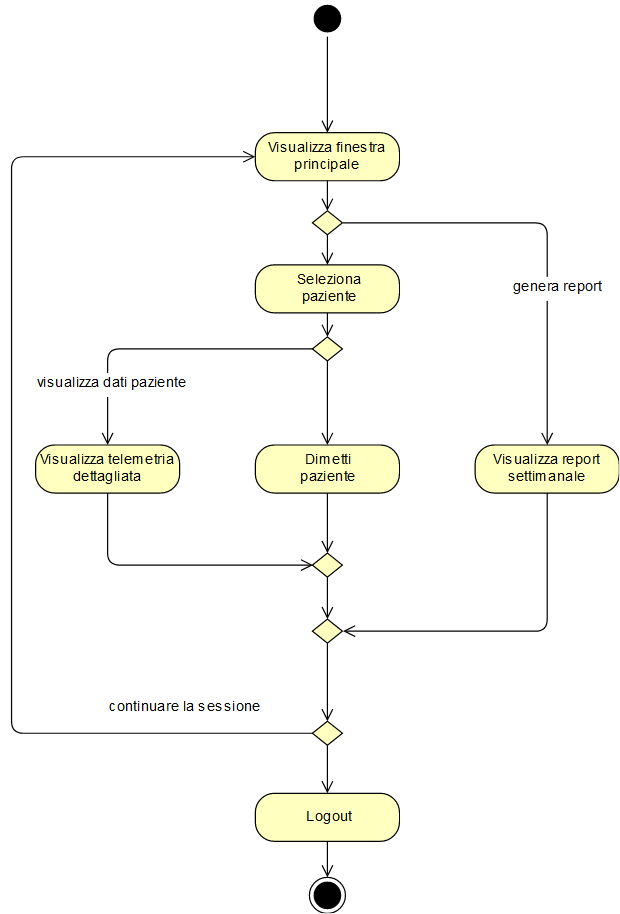
\includegraphics[scale=0.5]{activity/PrimarioActivity.png}
        \end{center}
            
            
\chapter{Sviluppo}
    \section{Tecnologie utilizzate}
        Agli albori del processo di sviluppo abbiamo deciso di usare il linguaggio di programmazione \textbf{Java}. Questo, infatti, implementa nativamente tutti gli strumenti che abbiamo utilizzato, quali input/output da file, threading e sincronizzazione.
        Abbiamo infine scelto di utilizzare il framework \textbf{Swing} per realizzare l'interfaccia grafica, in quanto di facile utilizzo e di eccellente portabilit\`a.\\
        
        Abbiamo adoperato metodi di sviluppo di tipo \textit{Agile}; il processo di sviluppo \`e stato diviso in finestre di tempo limitate chiamate iterazioni, con l'obiettivo di implementare ad ogni iterazione nuove funzionalit\`a pronte immediatamente al testing e seguente uso.\\
        
        La natura del lavoro di gruppo ci ha spinto ad adottare \textbf{Git} come software di controllo versione. Ne abbiamo beneficiato potendo delegare a un tool esterno la gestione dei files, comparare la stesura del codice in momenti separati e poter, in caso di errori, ritornare a versioni del software precedenti.
        I commit sono stati periodicamente pushati su un repository remoto hostato su \textbf{Github}.
        \begin{center}
                    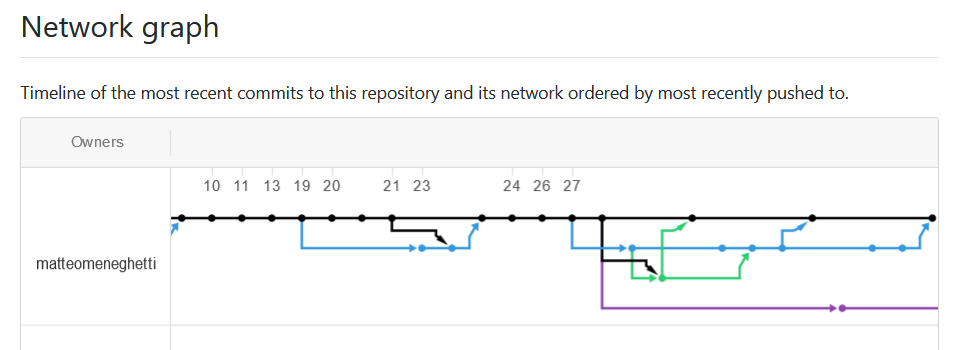
\includegraphics[scale=0.7]{immaginiVarie/networkGraph.png}
        \end{center}
        
        
    \section{Design Patterns utilizzati}
        \subsection*{Pattern architetturale}
            Il pattern architetturale scelto è il \textbf{MVC} (Model-View-Controller), supportato nativamente dal framework Swing. Il progetto \`e infatti separato in tre componenti principali:
            \begin{itemize}
                \item Model: corrisponde ai package data e analisi, i quali contengono le classi e le strutture dati adoperate dal sistema software.
                \item View: si trova interamente nel package gui, si occupa di gestire l'interazione visuale con l'utente.
                \item Controller: anche quest'ultima parte \`e localizzata nel package gui. Infatti, ogni classe ivi presente corrisponde a una finestra di dialogo, ognuna con compiti diversi da assolvere, quindi necessita di un listener di eventi ad hoc e con accesso personalizzato alle componenti.
            \end{itemize}
                \begin{center}
                    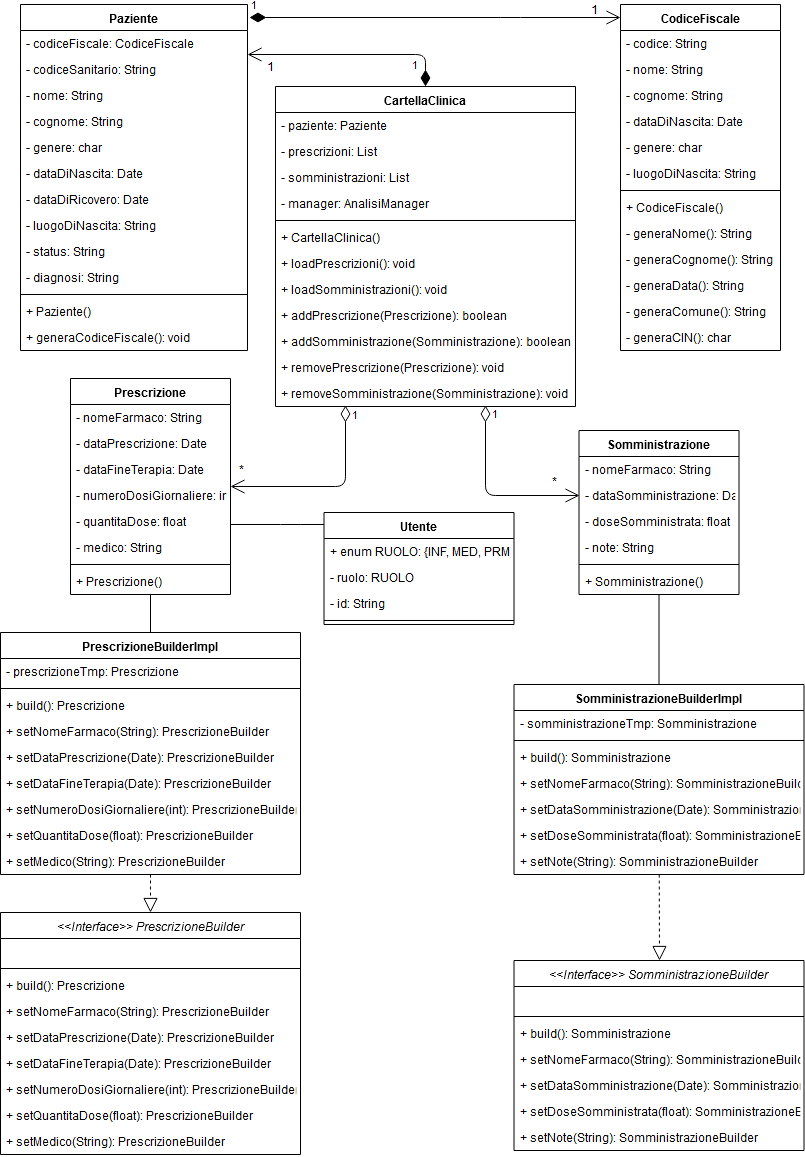
\includegraphics[scale=0.30]{class/DataPackage.png}
                \end{center}
                Da notare come la classe CartellaClinica sia l'hub centrale per accedere a tutti i dati rilevanti del paziente: l'anagrafica del paziente stesso, la lista di somministrazioni e prescrizioni.
                \begin{center}
                    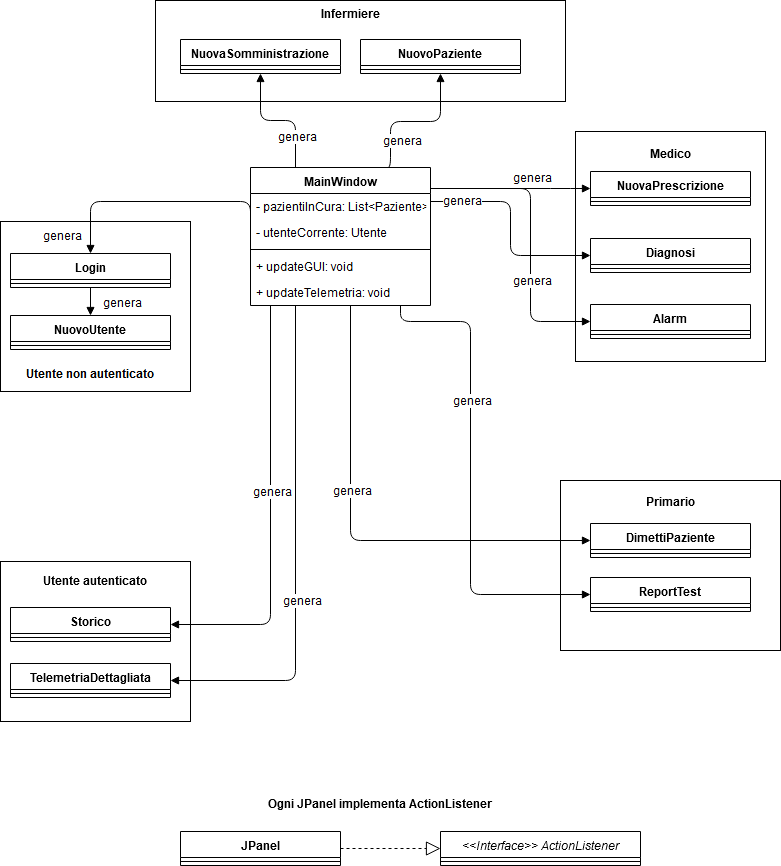
\includegraphics[scale=0.5]{class/GUIPackage.png}
                \end{center}
                \begin{center}
                    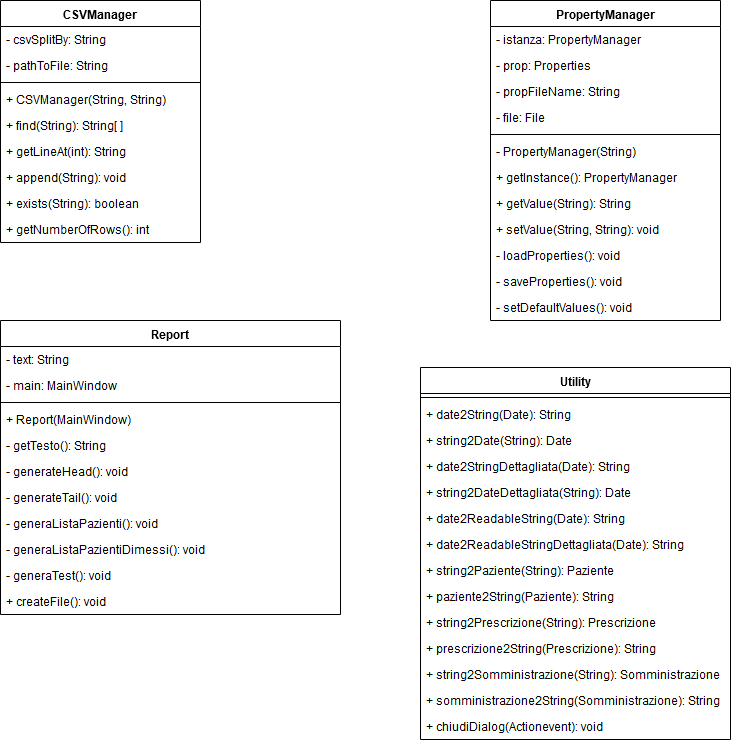
\includegraphics[scale=0.5]{class/UtilityPackage.png}
                \end{center}
    \newpage
        \subsection*{Pattern progettuali}
            Nota: si \`e cercato di non forzare l'utilizzo dei design patterns ma di attuarli con criterio dove ritenevamo necessario, in quanto offrono solidit\`a alla struttura del progetto e ne facilitano la lettura da parte di terzi. I pattern implementati sono i seguenti:
            \begin{itemize}
                \item Per il caricamento e il salvataggio delle propriet\`a \`e stata implementata una classe apposita nel package utility chiamata PropertyManager. Questa fornisce un wrapper per gestire la lettura e scrittura sul file .properties apposito. Per garantire che sia aperto solamente uno stream di input/output da file la classe PropertyManager implementa il pattern \textbf{singleton}. Il metodo getInstance() che garantisce l'accesso al singolo oggetto \`e invocato da un discreto numero di thread che scala linearmente con il numero di pazienti monitorati. Per questo nella firma del metodo lo si \`e definito come \textit{synchronized}.
                \item Le classi Prescrizione e Somministrazione descrivono il comportamento e le strutture dati atte a rappresentare rispettivamente una prescrizione scritta da un medico e una somministrazione eseguita da un infermiere. Il numero di argomenti dei costruttori di queste classi \`e pertanto elevato e risulta difficoltosa la lettura o rispettare l'ordine dei parametri durante l'invocazione. Per ovviare a queste difficolt\`a si \`e deciso di implementare il pattern \textbf{builder}, che garantisce un'interfaccia chiara e user-friendly per la creazione di oggetti.
                \item Come gi\`a anticipato, si \`e ritenuta critica l'astrazione e l'immediatezza per sincronizzare il Model con i dati presenti su disco. Come PropertyManager, anche la classe CSVManager offre diversi metodi per gestire file di estensione .csv, utilizzando metodi nativi delle librerie Reader e Writer di Java ma mascherandole al programmatore e fornendo uno strumento di assai pi\`u facile utilizzo. Lo si pu\`o considerare come un uso del \textbf{facade} pattern.
                \item Sono stati utilizzati pattern nativi di java, come l'\textbf{observer} per la gestione degli eventi generati dall'utente o l'\textbf{iterator}, fornito dall'implementazione di una qualunque List.
                \item Assai pi\`u interessante la generazione dei messaggi durante il monitoraggio dei pazienti. Un messaggio \`e un'istanza di una classe che implementa l'interfaccia Message. Ogni messaggio si differenzia dagli altri per il range dei valori che pu\`o assumere. Tuttavia il salvataggio dei messaggi su disco e la visualizzazione degli stessi deve essere medesima, quindi necessitavamo di creare oggetti di tipo diverso a runtime che per\`o si comportassero in modo simile. Il pattern \textbf{factory} \`e perfetto a questo scopo e la sua implementazione \`e il fulcro del package analisi.
                \begin{center}
                    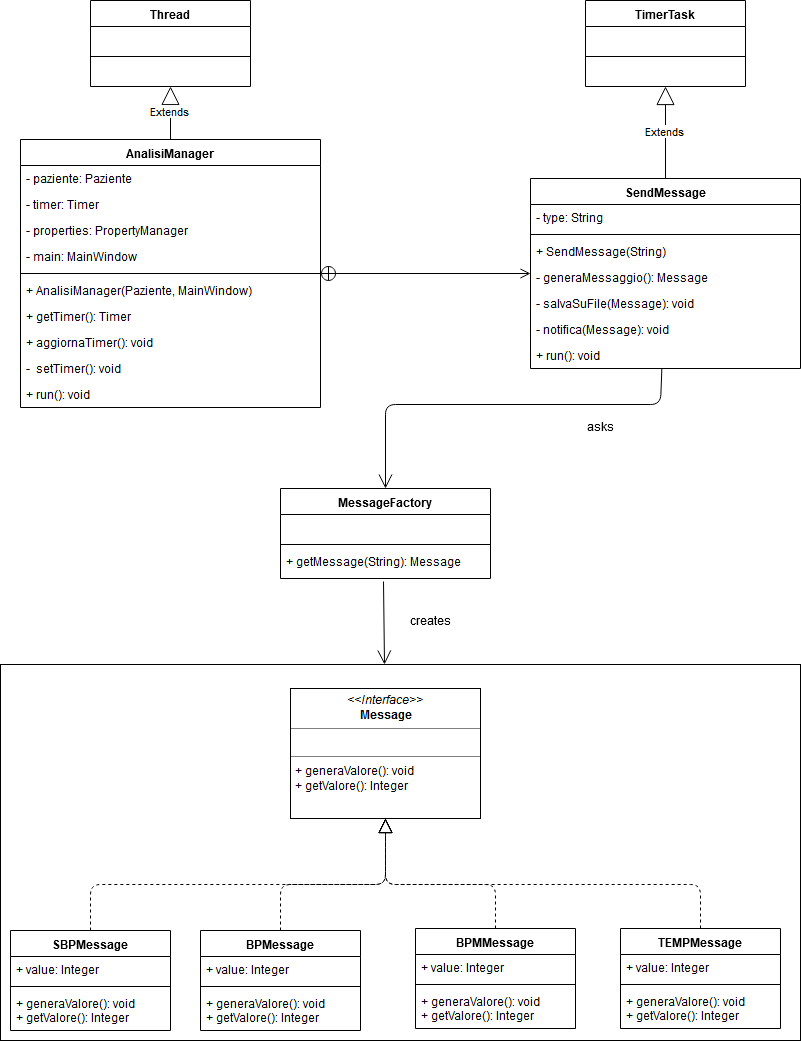
\includegraphics[scale=0.5]{class/AnalisiPackage.png}
                \end{center}
                \begin{center}
                    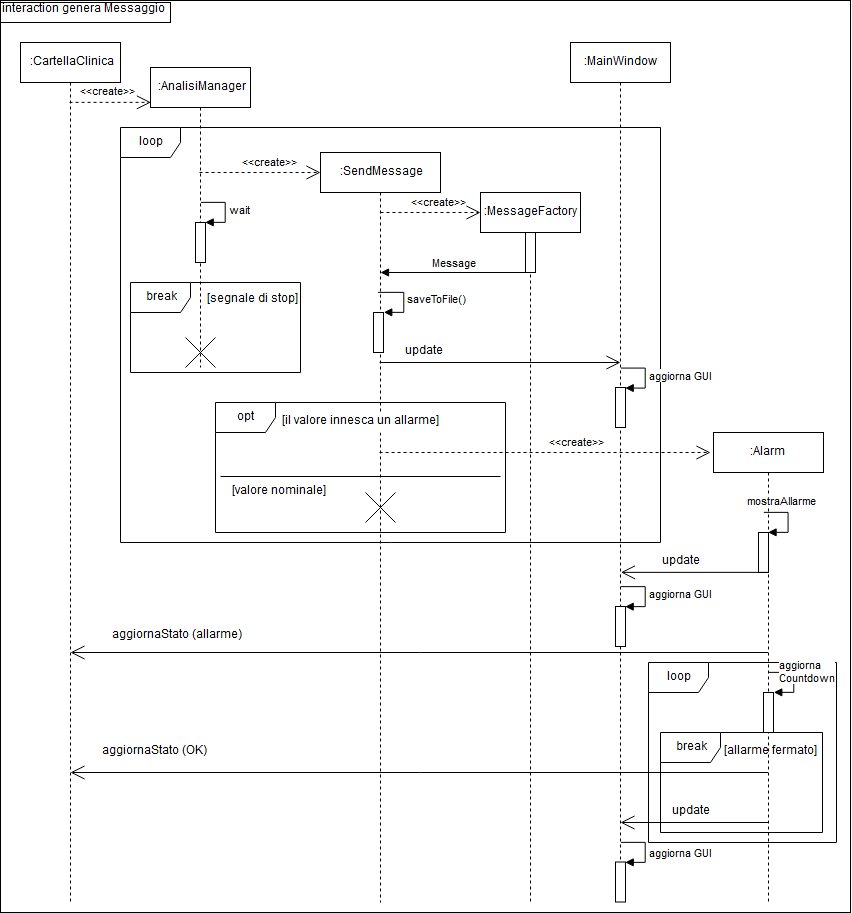
\includegraphics[scale=0.5]{sequence/MessageSequence.png}
                \end{center}
                
            \end{itemize}
\chapter{Test}
    \section*{Test Manuali}
        Per l'operazione di validazione e bug-fixing del software sono stati effettuati vari test da parte degli sviluppatori tra cui:
        \begin{itemize}
            \item Autenticazione con dati errati o mancanti PASSATO
            \item Controllo che ogni utente abbia accesso solamente alle funzioni a lui dedicate PASSATO
            \item Inserimento con dati mancanti di un nuovo paziente PASSATO
            \item Inserimento di una nuova prescrizione PASSATO
            \item Inserimento di una nuova somministrazione PASSATO
            \item Tentato inserimento di oltre 10 pazienti PASSATO
            \item Possibilit\`a di osservare dati del paziente in modalit\`a live PASSATO
            \item Impossibilit\`a di dimettere un paziente in stato critico PASSATO
            \item Generazione del file report.html PASSATO
            \item Cambiare i valori del file properties a runtime PASSATO
        \end{itemize}
        
    \subsection*{Test utenti esterni}
    Il software \`e stato fatto provare anche ad utenti al di fuori del ciclo di sviluppo. Sono stati dati loro indicazioni sulle operazioni che dovevano portare a compimento e nella maggioranza dei casi hanno portato a termine il loro compito. Nei casi rimanenti i problemi erano imputabili all'interfaccia, quindi ne \`e seguita una fase di analisi con lo scopo di renderla pi\`u intuitiva.

    \subsection*{Protocollo ARP: perché è stato introdotto?}
    Il protocollo
    

\end{document}
